%"###############################################
%
% Classification supervisée
%
%###############################################

% VAPOR: variables post-op à 12 mois
%
%###############################################

\subsubsection{VAPOR: IPSS à 12 mois}

L'arbre de régression présenté figure~\ref{fig-vapor-regtree-ipss12} infère la valeur la plus probable pour IPSS à 12 mois à partir d'une seule variable, le volume prostatique et indique la probabilité de chaque valeur constatée dans l'ensemble d'apprentissage, respectivement 1/2/3/4/6/14.

\begin{figure}[H]
\centering
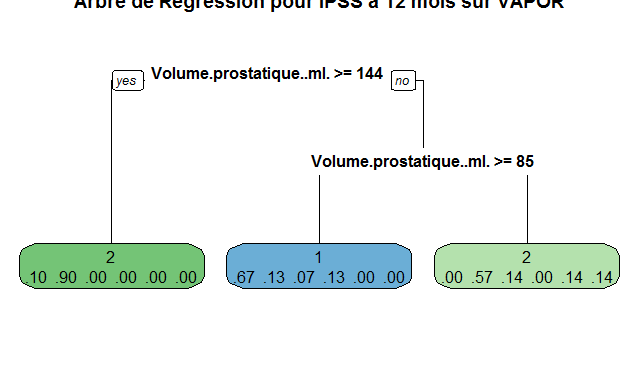
\includegraphics[width=0.75\textwidth]{../Fig/VAPOR/vapor-regtree-ipss12.png}
\caption{VAPOR: Arbre de régression pour IPSS à 12 mois}
\label{fig-vapor-regtree-ipss12}
\end{figure}

En appliquant cet arbre de régression sur l'ensemble de validation, nous obtenons une prédiction et une probablité des valeurs IPSS, illustrées figure~\ref{fig-vapor-regtree-predict-ipss12}.
 
\begin{figure}[H]
\centering
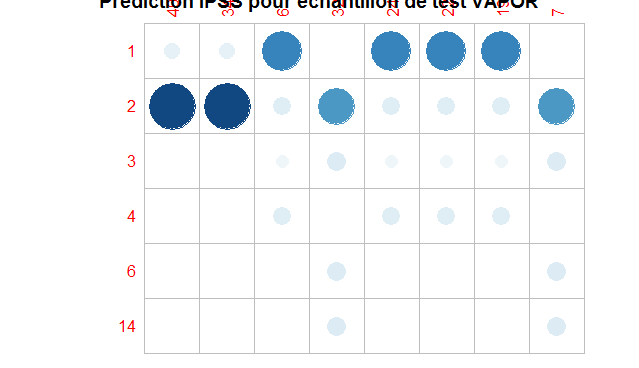
\includegraphics[width=0.75\textwidth]{../Fig/VAPOR/vapor-regtree-predict-ipss12.png}
\caption{VAPOR: Prévision pour IPSS à 12 mois}
\label{fig-vapor-regtree-predict-ipss12}
\end{figure}

La table de correspondance suivant nous permet d'évaluer ces résultats~:
\begin{lstlisting}[language=R]
> table(validation = testIPSS$IPSS__4, prediction =  predict(dt, testIPSS, type="class"))
          prediction
validation 1 2 3 4 6 14
        1  1 1 0 0 0  0
        2  1 2 0 0 0  0
        3  1 0 0 0 0  0
        4  1 0 0 0 0  0
        14 0 1 0 0 0  0
\end{lstlisting}
Soit un taux d'erreur de 62,5\%.

En utilisant une forêt aléatoire, plutôt qu'un unique arbre de régression, nous obtenons alors une
prédiction avec un taux d'erreur moindre, comme le montre cette nouvelle table de correspondance~:
\begin{lstlisting}[language=R]
> table(validation = testIPSS$IPSS__4, prediction =  predict(rf, testIPSS))
          prediction
validation 1 2 3 4 6 14
        1  2 0 0 0 0  0
        2  2 1 0 0 0  0
        3  1 0 0 0 0  0
        4  0 0 0 1 0  0
        14 0 0 0 0 1  0
\end{lstlisting}
Soit un taux d'erreur de 50\%.
        
\subsubsection{VAPOR: QoL à 12 mois}

\begin{figure}[H]
\centering
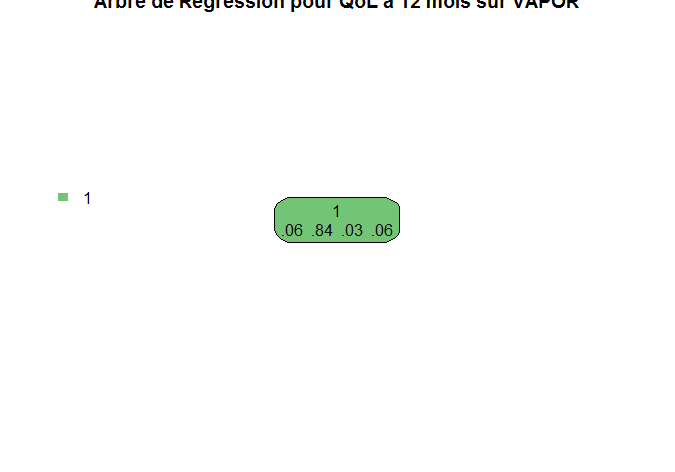
\includegraphics[width=0.75\textwidth]{../Fig/VAPOR/vapor-regtree-qol12.png}
\caption{VAPOR: Arbre de régression pour QoL à 12 mois}
\label{fig-vapor-regtree-qol12}
\end{figure}

\begin{figure}[H]
\centering
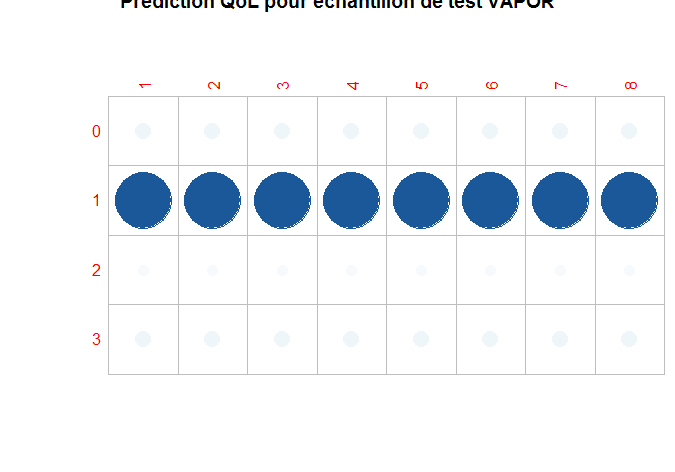
\includegraphics[width=0.75\textwidth]{../Fig/VAPOR/vapor-regtree-predict-qol12.png}
\caption{VAPOR: Prévision pour QoL à 12 mois}
\label{fig-vapor-regtree-predict-qol12}
\end{figure}

\begin{lstlisting}[language=R]
> table(validation = testQoL$QoL__4, prediction =  predict(dt, testQoL, type="class"))
          prediction
validation 0 1 2 3
         0 0 1 0 0
         1 0 6 0 0
         3 0 1 0 0
\end{lstlisting}
Soit un taux d'erreur de 25\%.

Afin d'améliorer ce taux d'erreur de prédiction, Nous utilisons une forêt aléatoire d'arbres de régression. Nous obtenons alors une nouvelle table de correspondance~:

\begin{lstlisting}[language=R]
> table(validation = testQoL$QoL__4, prediction =  predict(rf, testQoL))
          prediction
validation 0 1 2 3
         0 0 1 0 0
         1 0 6 0 0
         3 0 0 0 1
\end{lstlisting}
Soit un taux d'erreur de 12,5\%.


\subsubsection{VAPOR: Qmax à 12 mois}

L'arbre de régression obtenu pour la variable Qmax à 12 mois (colonne Qmax (ml/s)\_\_3) met en {\oe}uvre une seule variable (Cf. figure~\ref{fig-vapor-regtree-qmax12}). Les feuilles de l'arbre représentent, en première ligne, la valeur approximative pour Qmax à 12 mois. La ligne suivante indique le nombre de patients de l'échantillon d'apprentissage correspondant à cette feuille. 

\begin{figure}[H]
\centering
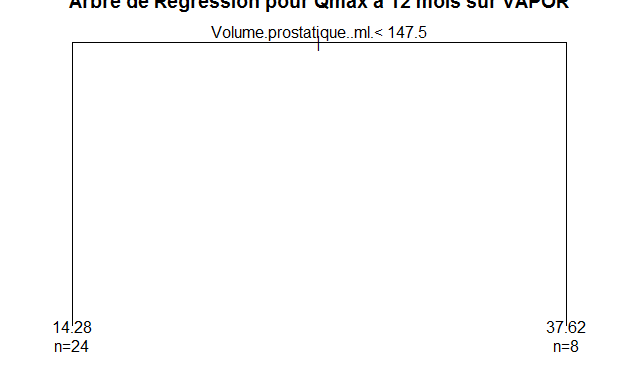
\includegraphics[width=0.75\textwidth]{../Fig/VAPOR/vapor-regtree-qmax12.png}
\caption{VAPOR: Arbre de régression pour Qmax à 12 mois}
\label{fig-vapor-regtree-qmax12}
\end{figure}

La figure~\ref{fig-vapor-regtree-test-qmax12} représente l'écart constaté entre valeurs prédites (colonne de gauche) et valeurs de référence (colonne de droite) sur l'échantillon de validation. La moyenne de ces écarts nous donne une mesure du taux d'erreur de l'arbre. En utilisant une forêt aléatoire d'arbres, figure~\ref{fig-vapor-forest-test-qmax12}, cet écart est réduit.

\begin{figure}[H]
\centering
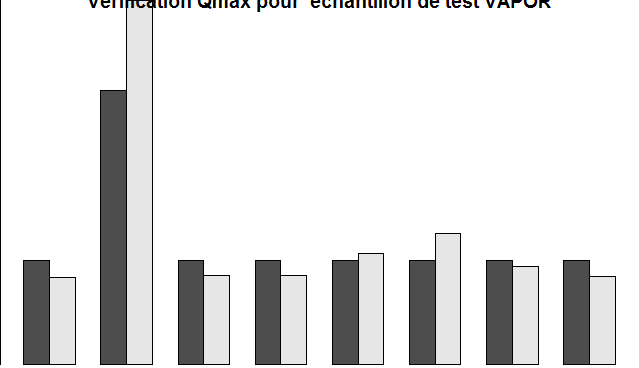
\includegraphics[width=0.75\textwidth]{../Fig/VAPOR/vapor-regtree-test-qmax12.png}
\caption{VAPOR: Evaluation des prévisions pour Qmax à 12 mois}
\label{fig-vapor-regtree-test-qmax12}
\end{figure}

\begin{figure}[H]
\centering
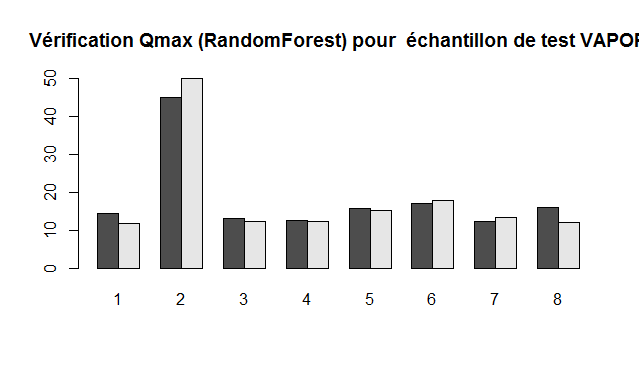
\includegraphics[width=0.75\textwidth]{../Fig/VAPOR/vapor-forest-test-qmax12.png}
\caption{VAPOR: Evaluation des prévisions (Random Forest) pour Qmax à 12 mois}
\label{fig-vapor-regtree-test-qmax12}
\end{figure}

